\documentclass[beamer=true]{standalone}
\usepackage{../../preamblesnotes}

%Information to be included in the title page:
\title{第三課}
\author{力的轉動效應 Turning effect of forces}
\institute{周末班}
\date{}

\begin{document}
\frame{\titlepage}


\begin{frame}{力矩Moment of force/ torque}
    \begin{itemize}
        \item 在剛體(有固定形狀和大小的物體)中,力能令剛體圍繞一點轉動。\\
              In a rigid body (an object with a fixed shape and size), forces can let a rigid body  rotate about a point.
        \item 作用力促使物體繞著支點轉動的趨向。\\Tendency of rotation on a pivot by an external force.
    \end{itemize}\bigskip
    {\par\centering
        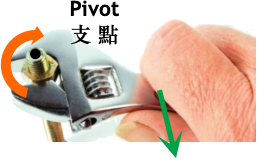
\includegraphics[width=.4\textwidth]{assets/76cf8376.png}
        \par}
\end{frame}
\begin{frame}{力矩Moment of force}
    \begin{itemize}
        \item 力矩是\textbf{矢量},單位是牛頓米(N m)。\\Torques are \textbf{vectors}, its unit is Newton-meter (N m).
        \item 力矩的\textbf{方向}可以是順時針或逆時針,視乎它會令物體向哪個方向轉動。\\The \textbf{directions} of torques can be clockwise or anti-clockwise, it depends on how the force spins the object.
        \item 力矩(moment of force)又稱轉矩(turning moment)。
        \item 而支點(pivot) 又稱支軸或轉動軸心。
    \end{itemize}

\end{frame}

\begin{frame}{力矩moment of force}
    \begin{exampleblock}
        {力矩量值magnitude of moment of force}
        \begin{equation}
            \tau = d\times F
        \end{equation}
    \end{exampleblock}
    \begin{itemize}
        \item $\tau$ [\unit{N.m}] = 力矩。Torque.
        \item F [N] = \textbf{施力}。\textbf{Applied force}.
        \item d  [m] = 施力至支點的\textbf{垂直距離}。\\ \textbf{Perpendicular distance} of applied force from the pivot.
    \end{itemize}
    {\par\centering
    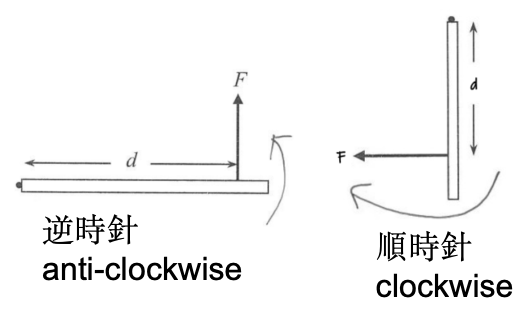
\includegraphics[width=0.5\textwidth]{assets/8db14dd2.png}
    \par}
\end{frame}

\begin{frame}{力矩moment of force}
    當力矩的方向和剛體的幾何產生角度時,力矩的公式需要加上一個 $\sin\theta$來表達。\\When the direction of the torque is at an angle to the geometry of the object, the formula for torque needs to include an additional $\sin\theta$ term.
    \begin{alertblock}
        {力矩量值magnitude of moment of force}
        \begin{equation}
            \tau = d\times F \times\sin \theta
        \end{equation}
    \end{alertblock}
    \bigskip
    {\par\centering
        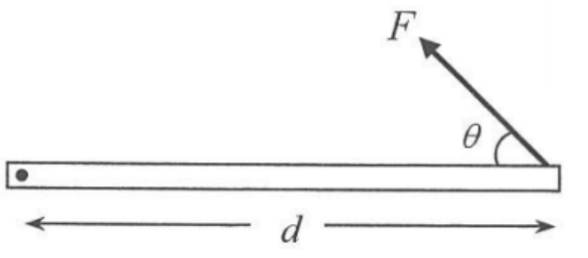
\includegraphics[width=.4\textwidth]{assets/dfd826ba.png}
        \par}
\end{frame}

\begin{eg}
    對於以下各力的系統中,求對 O 的\textbf{合力矩量值}及\textbf{方向}。 \\For each of the following systems of force, find the \textbf{magnitude} and the \textbf{direction} of \textbf{resultant moment} about O.
        {\par\centering
            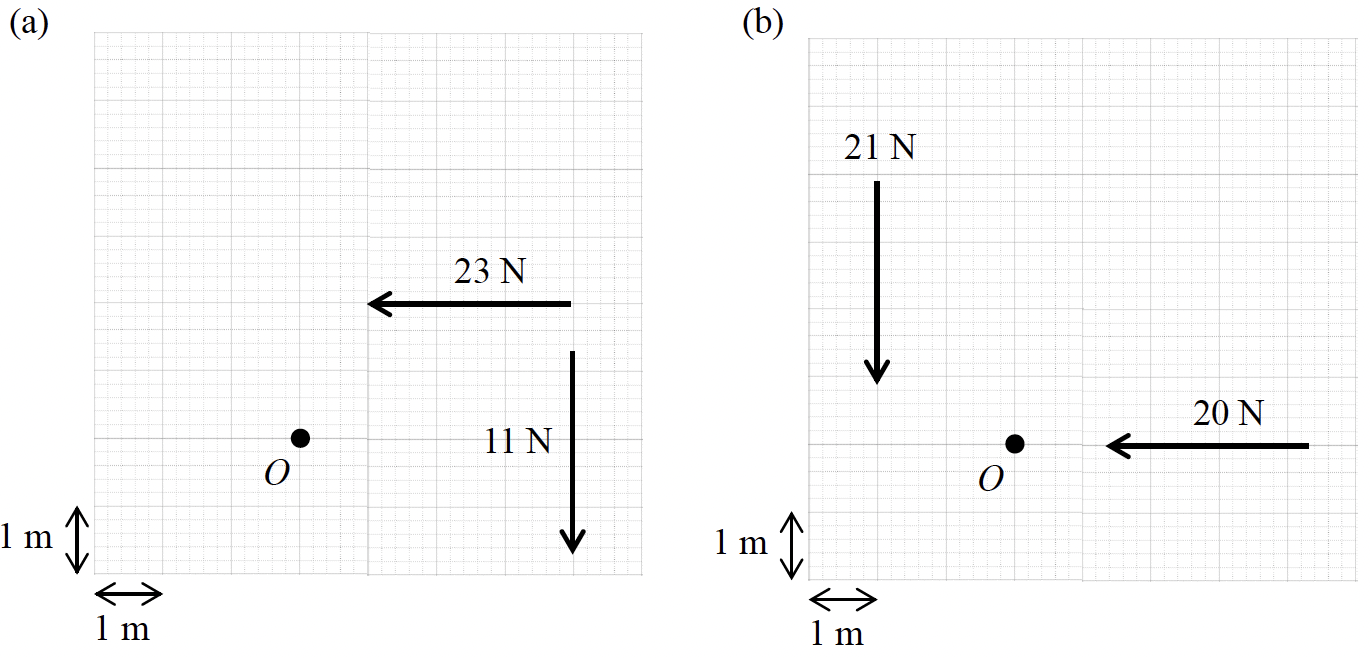
\includegraphics[width=\textwidth]{assets/a1fab181.png}
            \par}
\end{eg}
\begin{eg}
    對於以下各力的系統中,求對 O 的\textbf{合力矩量值}及\textbf{方向}。 \\For each of the following systems of force, find the \textbf{magnitude} and the \textbf{direction} of \textbf{resultant moment} about O.
        {\par\centering
            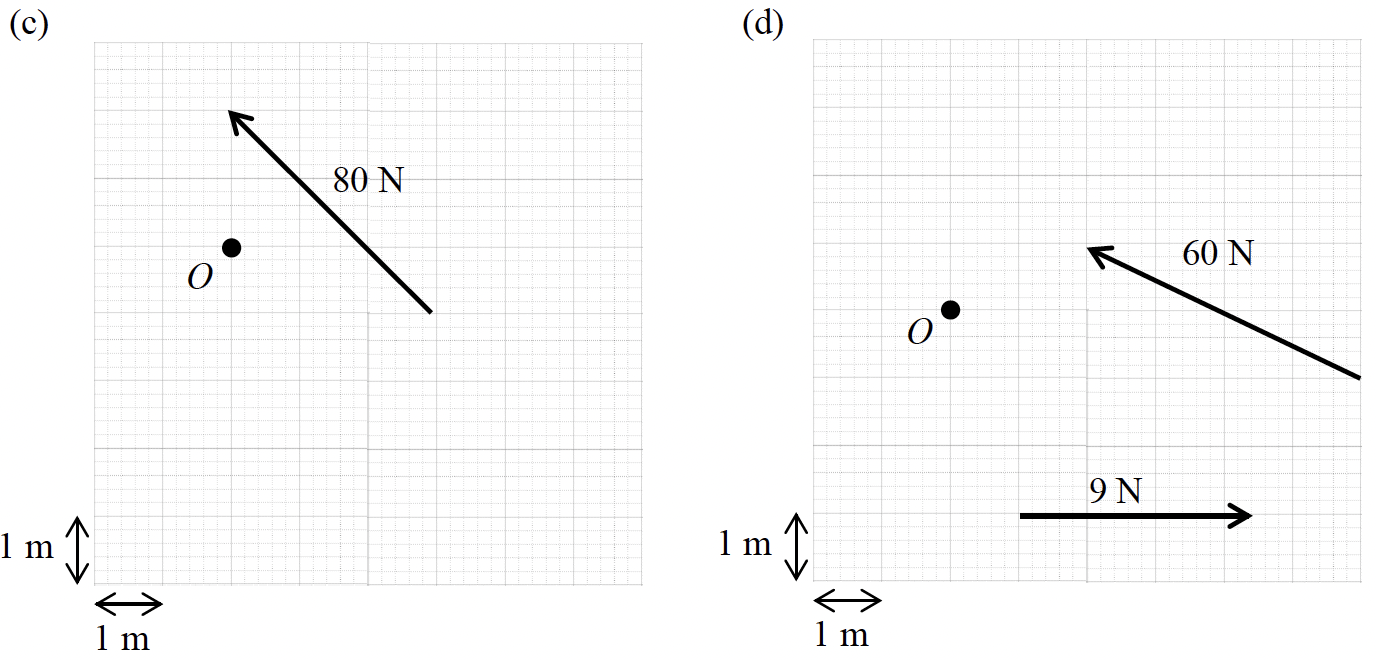
\includegraphics[width=\textwidth]{assets/d462b1fc.png}
            \par}
\end{eg}


\begin{frame}{剛體平衡Rigid body equilibrium}
    \begin{itemize}
        \item 平移平衡 Translational equilibrium
              \begin{itemize}
                  \item 淨力 Net Force = 0
              \end{itemize}
    \end{itemize}
    {\par\centering
    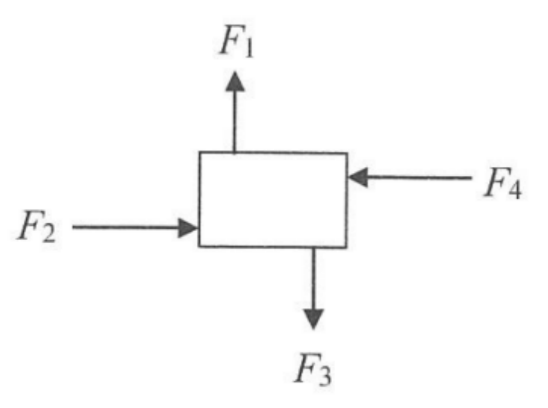
\includegraphics[width=.45\textwidth]{assets/e0f98693.png}

    \par}

\end{frame}
\begin{frame}{剛體平衡Rigid body equilibrium}
    \begin{itemize}
        \item 旋轉平衡Rotational equilibrium
              \begin{itemize}
                  \item 淨力矩Net torque = 0
              \end{itemize}
    \end{itemize}
    {\par\centering
    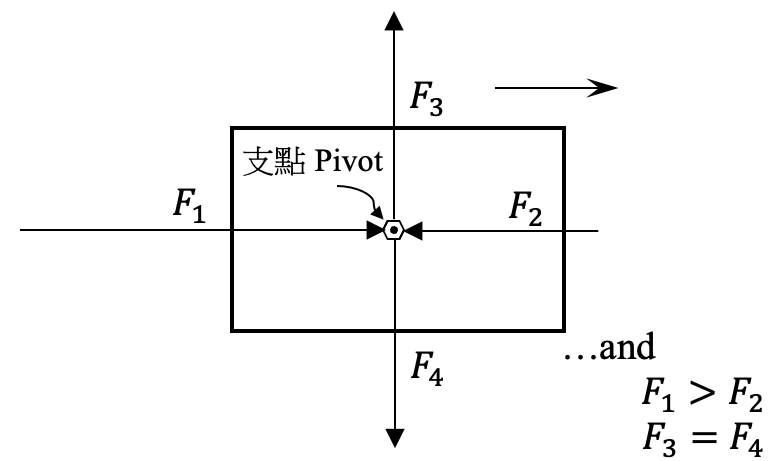
\includegraphics[width=.5\textwidth]{assets/4eeeca69.png}
    \par}

\end{frame}
\begin{frame}{剛體平衡Rigid body equilibrium}
    \begin{itemize}
        \item \textbf{平衡}狀態或\textbf{靜止}狀態:\\\textbf{Equilibrium} or \textbf{at rest}:
    \end{itemize}\bigskip
    \begin{columns}
        \column{.4\textwidth}

        \begin{longtblr}[
            label = none,
            entry = none,
            ]{
            width = \linewidth,
            colspec = {Q[56]Q[833]},
            cells = {c},
            cell{1}{1} = {r=3}{},
            }
            = & 平移平衡 Translational equilibrium \\
              & +                              \\
              & 旋轉平衡Rotational equilibrium
        \end{longtblr}

        \column{.4\textwidth}
        {\par\centering
            
\includegraphics[width=0.66\textwidth]{assets/0a37d983.png}
            \par}

    \end{columns}
\end{frame}


\begin{frame}{重心Center of gravity}
    \begin{itemize}
        \item 每個剛體都有一個稱為重心(簡稱CG)的固定點,剛體的全部重量好像都作用於這一點。\\Every rigid body has a fixed point called the centre of gravity (abbr. C.G.), where the object's weight seems to act at.
    \end{itemize}\bigskip
    {\par\centering
        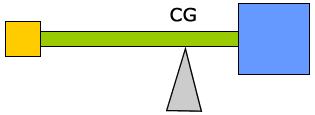
\includegraphics[width=0.5\textwidth]{assets/ad409000.png}
        \par}
\end{frame}
\begin{frame}{重心Center of gravity}
    \begin{itemize}
        \item 均勻且對稱的物體(例如密度和直徑都恆定不變的棒),重心位於它的中心,至於不規則物體的重心,則可用實驗方法找出。\\A uniform and symmetric object (e.g. a rod with uniform density and cross-section) has its C.G. at its centre, while the C.G. of an irregular object can be determined experimentally.
    \end{itemize}\bigskip
    {\par\centering
        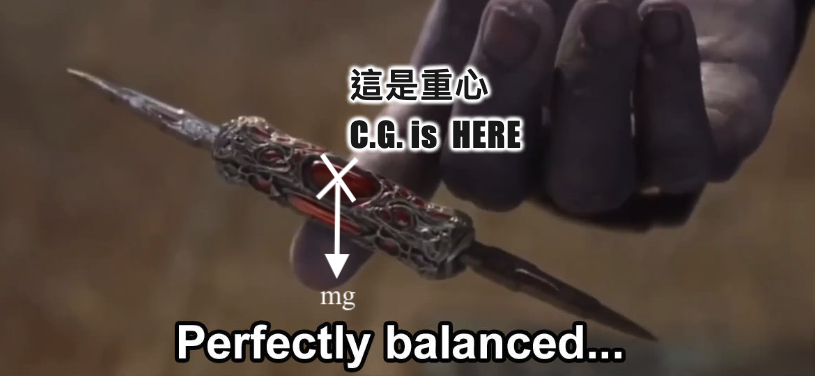
\includegraphics[width=0.66\textwidth]{assets/0610c65e.png}
        \par}
\end{frame}


\begin{frame}{力矩題目計算步驟Steps for problems}
    \begin{enumerate}
        \item 畫出自由體圖。\\Draw the free body diagram.
        \item 選擇合適的支點。\\Choose a suitable pivot for calculation.
        \item 平衡順時針和逆時針的力矩。\\Balance clockwise and counter-clockwise moments.
        \item 平衡不同方向的力。\\Balance forces of different directions.
    \end{enumerate}
\end{frame}
\begin{frame}{如何選擇合適的支點How to choose a suitable pivot}
    \begin{itemize}
        % \setlength{\itemsep}{0.5cm}
        \item 在平衡狀態下,可以選擇任何一點作為支點。\\In equilibrium state, any point can be chosen as pivot point.
              \begin{itemize}
                  \item 計算過程中,所有通過支點作用的力會被忽略掉。\\All forces acting through pivot will be ignored in the calculation process.
              \end{itemize}
        \item 在旋轉狀態下,只能選擇旋轉的支點進行計算。\\In rotating state, only the pivot of rotation can be chosen for calculation.
    \end{itemize}
\end{frame}



\begin{eg}
    一塊質量可略的板水平放置在支撐點上。板上如圖放上質量分別為 4 kg 和 $m$ 的小方塊後,仍保持水平。4 kg 與支撐點相距 80 cm,$m$ 與支撐點相距 32 cm。\\A wooden plank with negligible mass is put on a support. After putting a mass of 4 kg and $m$ are put on the plank, the plank still keeps horizontal. The distance between the 4 kg and the support is \qty{80}{cm}, that between $m$ and the support is 32 cm.
        {\par\centering
            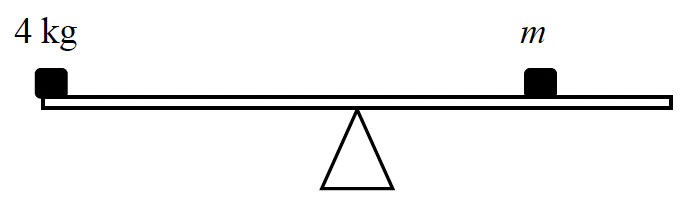
\includegraphics[width=.4\textwidth]{assets/b025a484.png}
            \par}

\end{eg}

\begin{eg}
    \begin{itemize}
        \item [(a)] 求 $m$ 的值。 \\Find the value of $m$.
    \end{itemize}
\end{eg}

\begin{eg}
    \begin{itemize}
        \item [(b)]求支撐點對板施加的力的量值。 \\Find the magnitude of the force acting on the plank by the support.
    \end{itemize}
\end{eg}

\begin{eg}
    圖中的梯子 XY 長 3 m,質量為 5 kg,斜倚牆上靜止不動,X 點離地 2 m。假設梯子是均質,且牆壁與梯子之間的摩擦力可略去不計。\\The ladder XY in the figure has a length and mass of 3 m and 5 kg respectively, it leans on the wall and stays at rest, point X is 2 m from the ground. Assume the ladder is uniform and assume negligible friction between the wall and the ladder.
        {\par\centering
            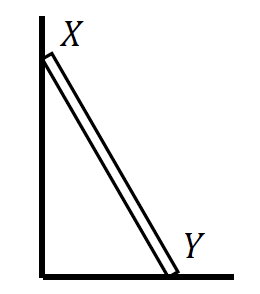
\includegraphics[width=.25\textwidth]{assets/0ba0e131.png}
            \par}
    \begin{itemize}
        \item [(a)] 繪畫梯子的隔離體圖。\\Sketch the free-body diagram of the ladder.
    \end{itemize}
\end{eg}
\begin{eg}
    \begin{itemize}
        \item [(b)] 設地面作用於梯子的合力為 R,求 R 的量值和方向。\\Let the resultant force acting on the ladder be R, find the magnitude and direction of R.
    \end{itemize}
\end{eg}

\begin{eg}
    一根質量為 8 kg 的勻質木棒其中一端光滑鉸接在牆上,另一端以輕繩如圖懸掛。繩與水平之間的夾角是 \dg{20}。在木棒上掛上一個質量為 5 kg 的物件。 \\A uniform wooden rod with mass 8 kg is hinged smoothly at one end on the wall and is hung by a light thread on the wall at the other end as shown. The thread is \dg{20} above horizontal. A 5 kg object is hung on the rod.
        {\par\centering
            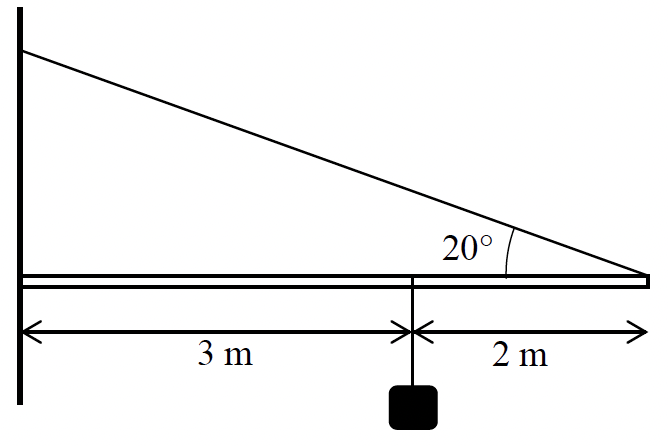
\includegraphics[width=.35\textwidth]{assets/b6070d24.png}
            \par}
    求繩子及牆壁對木棒施加的力的量值。 \\Find the magnitudes of the forces acting on the rod.
\end{eg}
\begin{eg}
    \begin{itemize}
        \item [sol.]
    \end{itemize}
\end{eg}

\begin{frame}{力偶Couples}
    \begin{itemize}
        \item 只有淨力矩,沒有淨力。\\There is only net moment, no net force.
        \item 物體只會在原地打轉,不會平移移動。\\The object will only rotate in place, it will not undergo translational motion.
    \end{itemize}\bigskip

    {\par\centering
        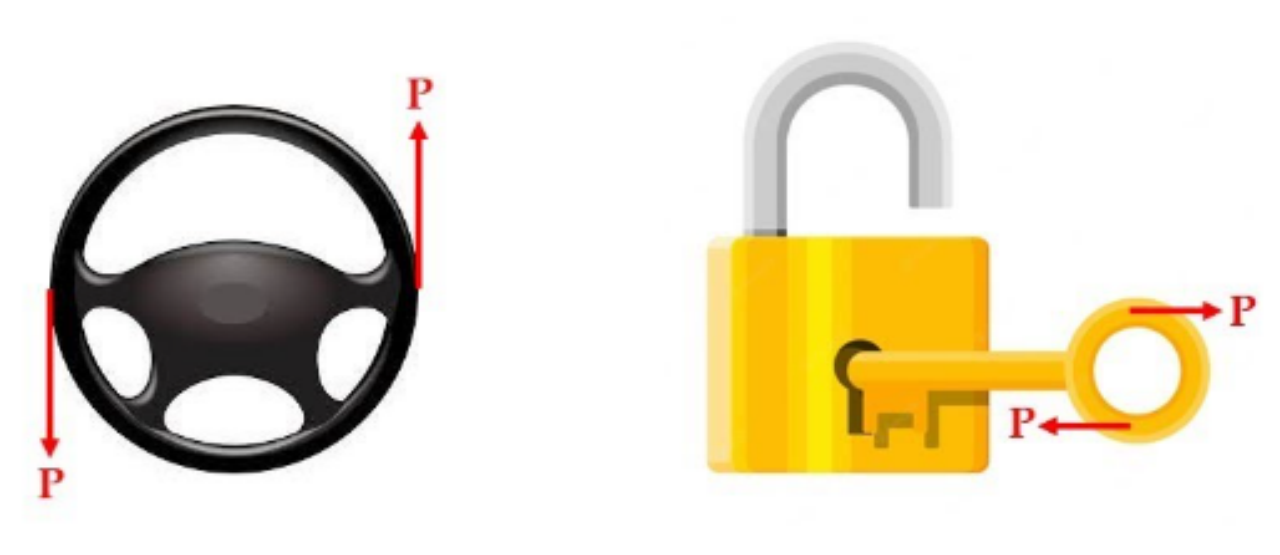
\includegraphics[width=.5\textwidth]{assets/88b4eb5e.png}
        \par}
\end{frame}
\begin{frame}{力偶Couples}
    \begin{alertblock}
        {力偶的淨力矩Net moment of couples}
        \begin{equation}
            \tau = d\times F
        \end{equation}
    \end{alertblock}

    {\par\centering
    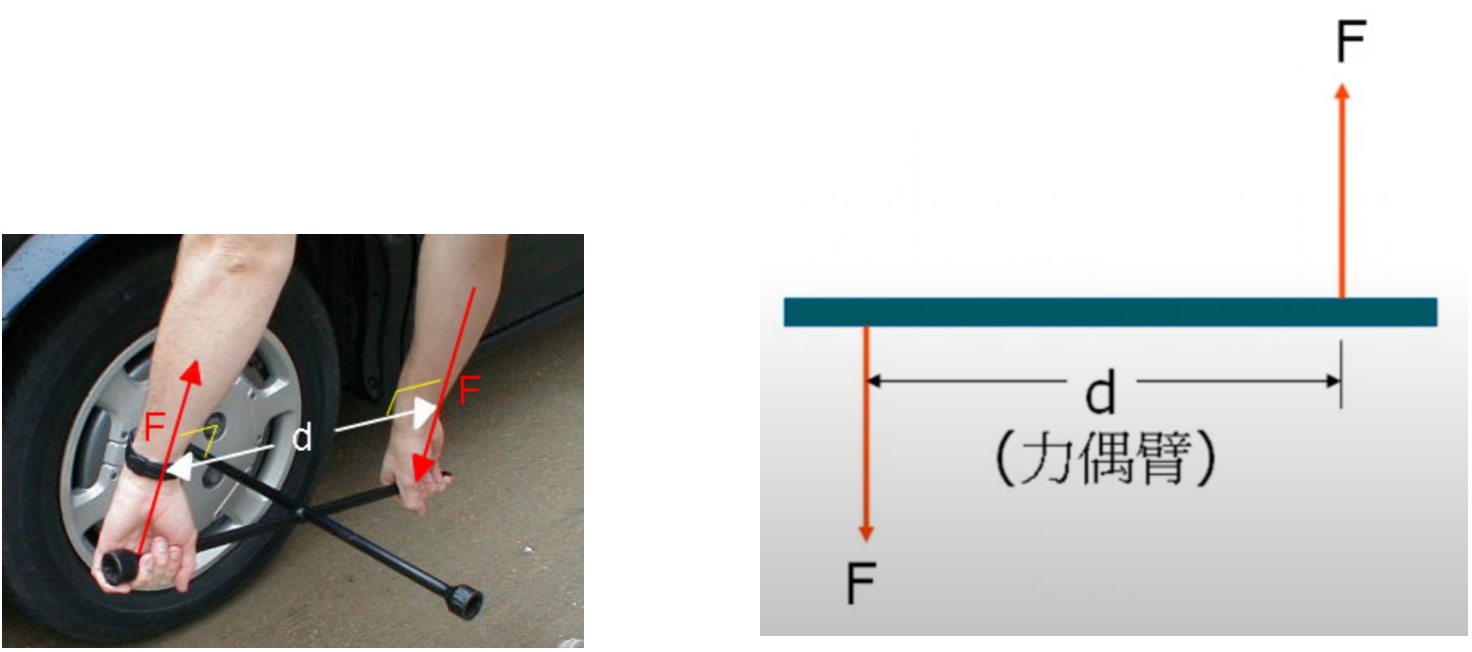
\includegraphics[width=0.8\textwidth]{assets/9168cf9b.png}
    \par}
\end{frame}
\begin{frame}{力偶Couples}
    \begin{itemize}
        \item d 越大,所需要的 F 越小。\\As d increases, the required F decreases.
    \end{itemize}\bigskip
    {\par\centering
        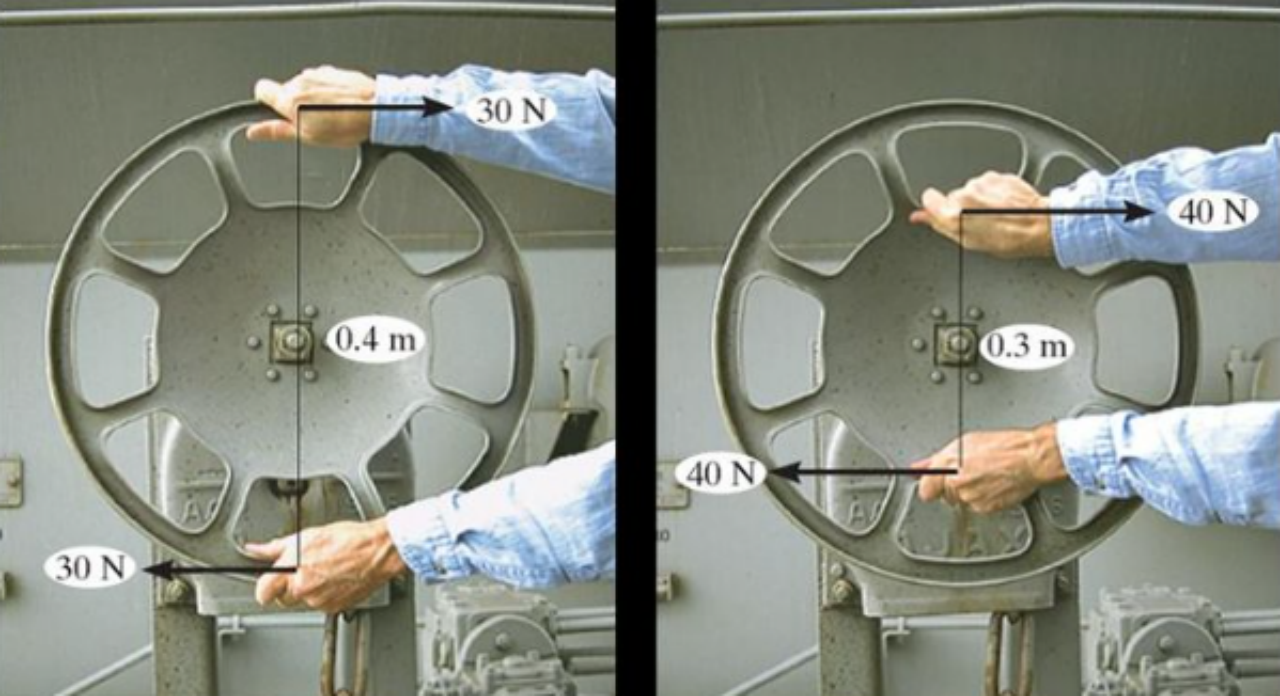
\includegraphics[width=0.8\textwidth]{assets/347900c8.png}
        \par}
\end{frame}


\begin{frame}{找重心的一些方法Methods to find C.G.}
    \begin{itemize}
        \item 找對稱特徵 (幾何中心) By symmetry (Geometric center)
        \item 鉛垂線 Using plumb lines
        \item 計算出來By calculation (不考Out-syl)
    \end{itemize}

\end{frame}
\begin{frame}{找對稱特徵By symmetry}
    \par{\par\centering
        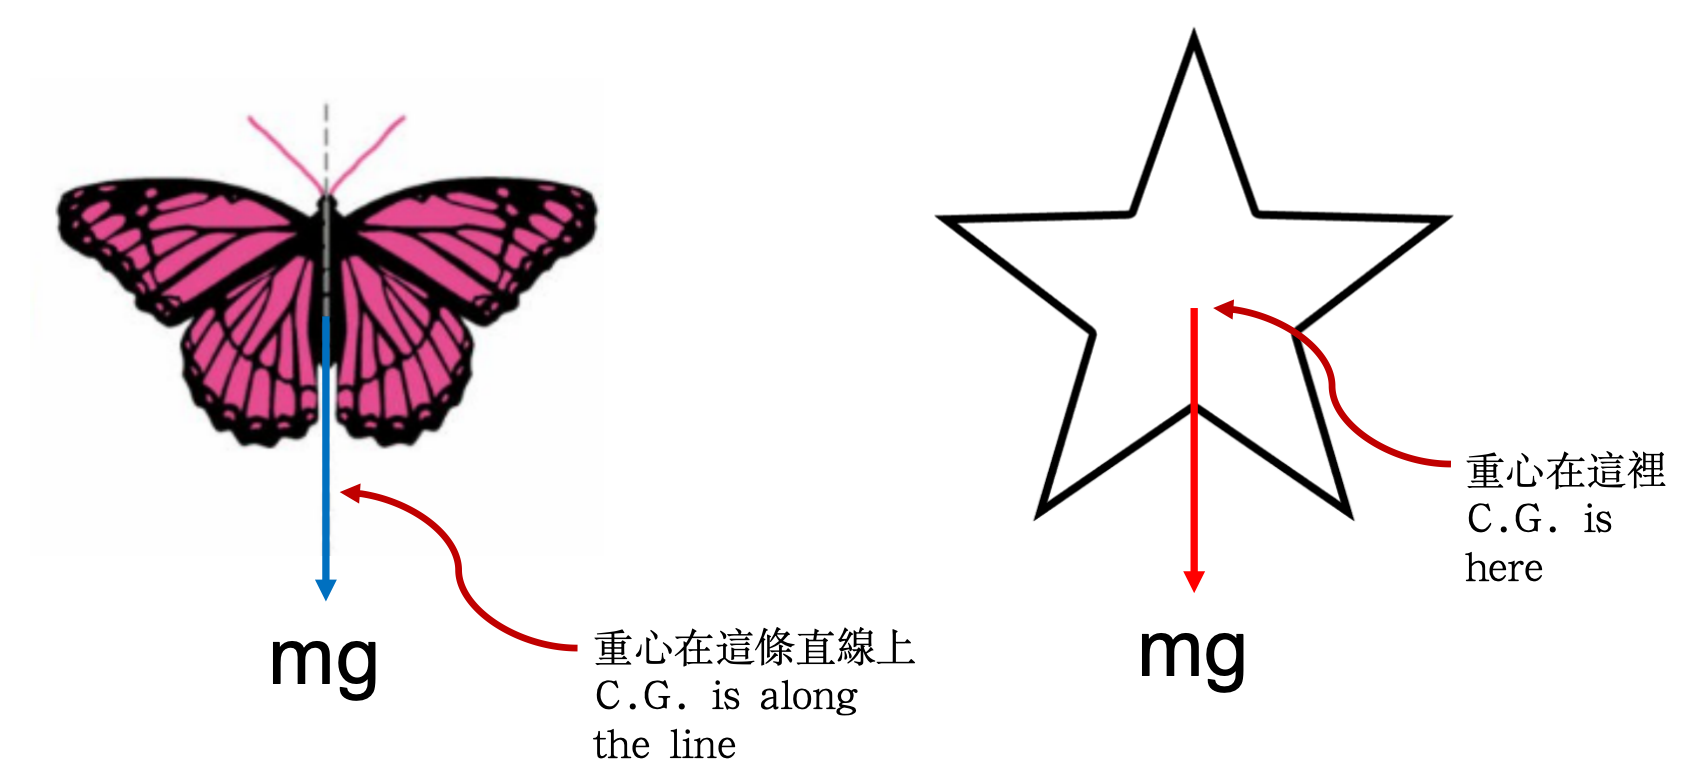
\includegraphics[width=\textwidth]{assets/78bde2e5.png}
        \par}
\end{frame}

\begin{frame}{鉛垂線 Using plumb lines}
    \begin{columns}
        \column{.5\textwidth}
        \begin{itemize}
            \item 把鉛垂線懸掛在點 A。\\Hang the plumb line at point A.
            \item 重心必須在線上的某一點。\\The center of gravity must be at a certain point on the line.
            \item 旋轉物件,把鉛垂線懸掛在另一點 C。\\Rotate the object, hang the plumb line at another point C.
            \item 重心 = 兩條線的交點。\\The center of gravity = the intersection point of the two lines.
        \end{itemize}



        \column{.5\textwidth}
        {\par\centering
            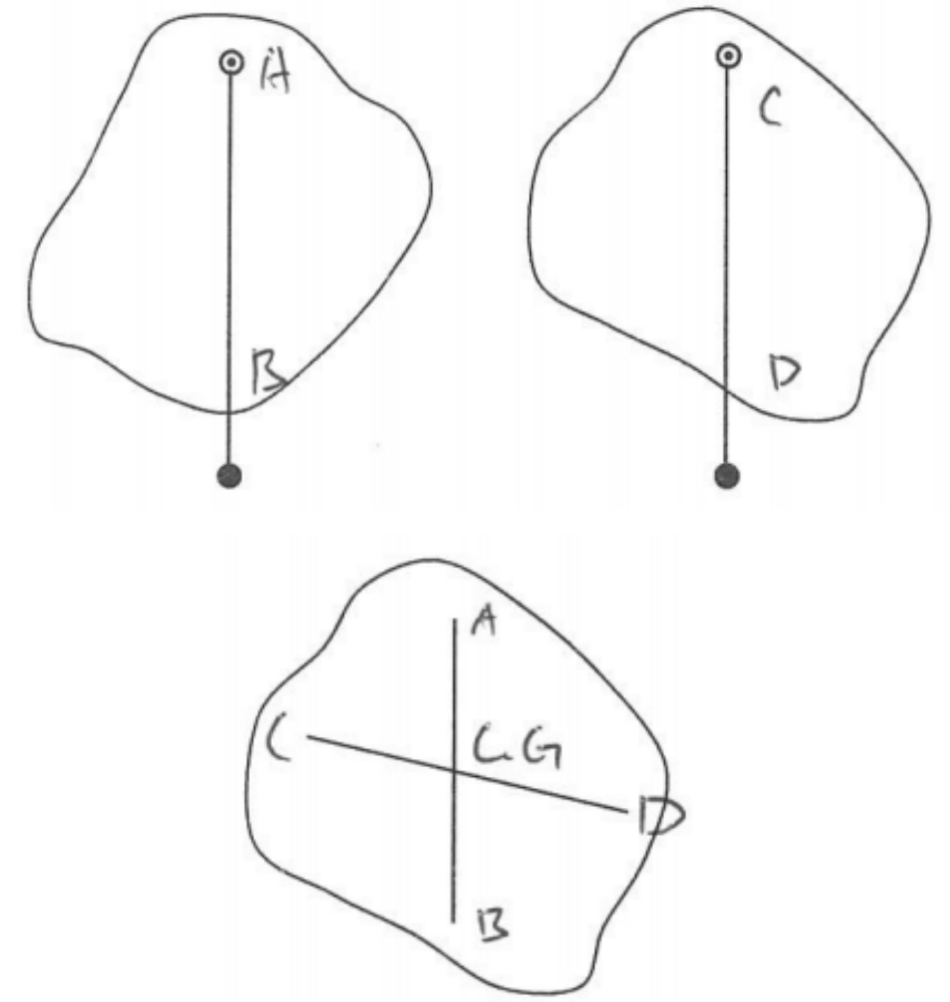
\includegraphics[width=\textwidth]{assets/85f02607.png}
            \par}
    \end{columns}
\end{frame}

\begin{frame}{鉛垂線 Using plumb lines}
    \begin{columns}
        \column{.5\textwidth}
        \begin{itemize}
            \item 把鉛垂線懸掛在點 A。\\Hang the plumb line at point A.
            \item 重心必須在線上的某一點。\\The center of gravity must be at a certain point on the line.
            \item 旋轉物件,把鉛垂線懸掛在另一點 C。\\Rotate the object, hang the plumb line at another point C.
            \item 重心 = 兩條線的交點。\\The center of gravity = the intersection point of the two lines.
        \end{itemize}



        \column{.5\textwidth}
        {\par\centering
            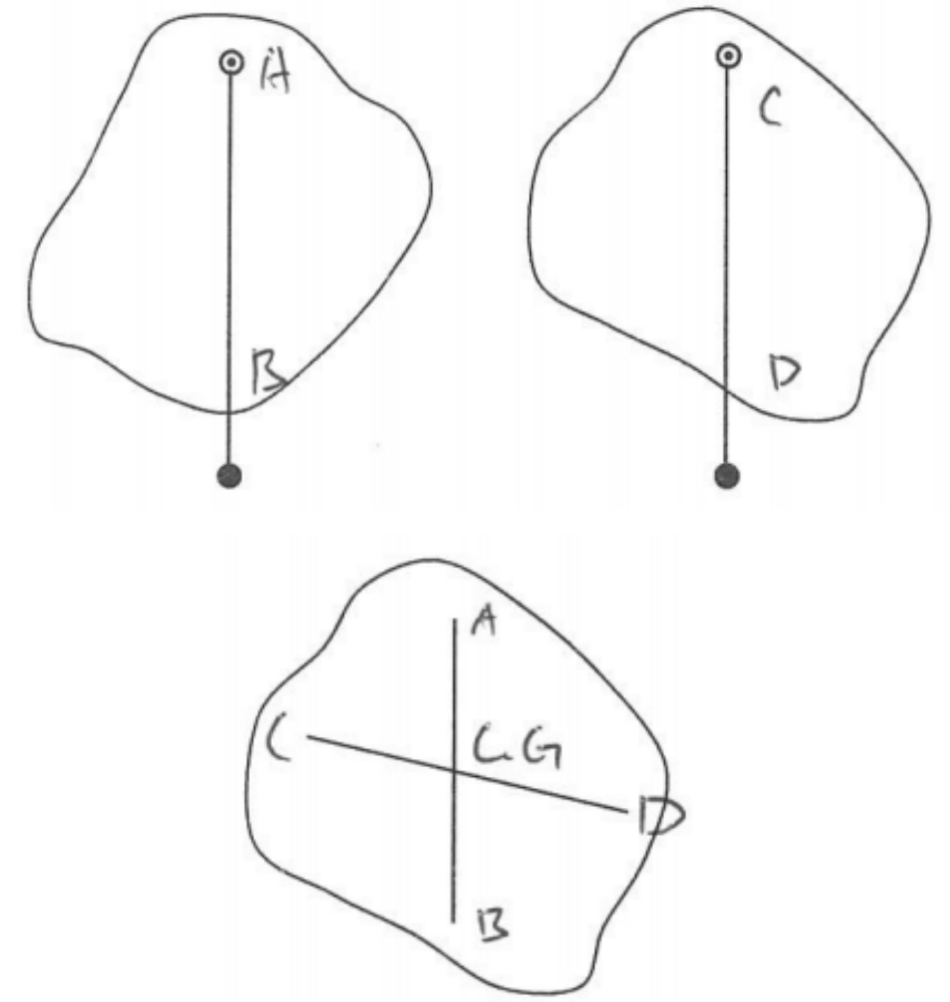
\includegraphics[width=\textwidth]{assets/85f02607.png}
            \par}
    \end{columns}
\end{frame}

\begin{frame}{直接計算出來By calculation (Out-syl)}
    \textbf{不考不考不考}:
    {\par\centering
    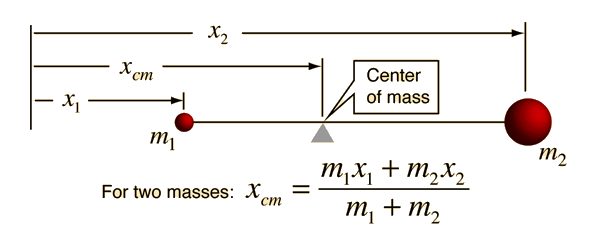
\includegraphics[width=0.5\textwidth]{assets/aae43746.png}
    \par}
    {\par\centering
    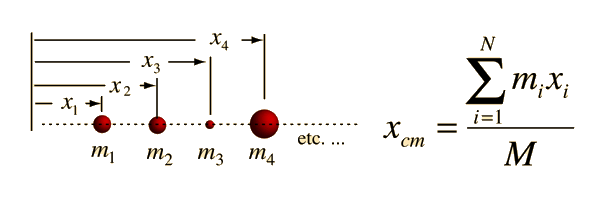
\includegraphics[width=0.5\textwidth]{assets/23195dc5.png}
    \par}
    {\par\centering
    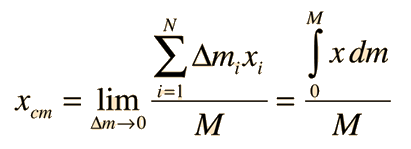
\includegraphics[width=0.4\textwidth]{assets/14123e56.png}
    \par}
\end{frame}

\begin{frame}{平衡狀態的穩定性 Equilibrium stability}
    \begin{itemize}
        \item 給予一個小的推力,穩定平衡會趨向回到原始位置,而不穩定平衡則會傾倒。\\Given a small push, a stable equilibrium would tend to go back to its original position, while unstable equilibrium would topple.
    \end{itemize}\bigskip
    {\par\centering
        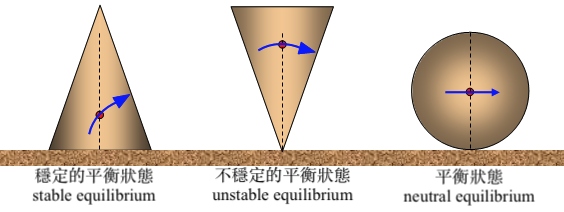
\includegraphics[width=.8\textwidth]{assets/84b8e1a5.png}
        \par}
\end{frame}
\begin{frame}{平衡狀態的穩定性 Equilibrium stability}
    \begin{itemize}
        \item 一般而言,可以通過增加底座尺寸和降低重心位置來提高穩定性。\\In general, better stability can be achieved by increasing the base size and decreasing the C.G. position.
    \end{itemize}
    %    {\par\centering
    % 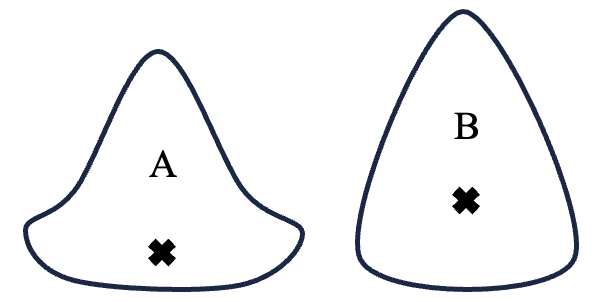
\includegraphics[width=0.66\textwidth]{assets/5f31a348.png}
    % \par}
    \begin{figure}
        \centering
        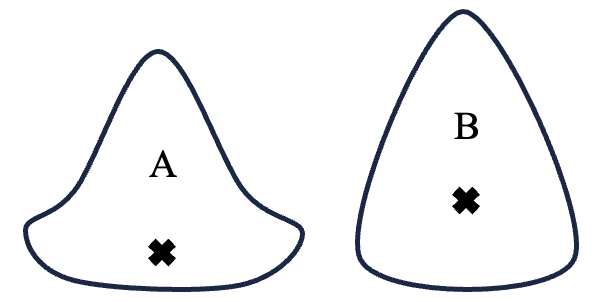
\includegraphics[width=0.66\textwidth]{assets/5f31a348.png}
        \caption{A比B更不容易被推倒,因為A具有較大的底座和較低的重心。A is more difficult to topple than B because of its larger base and lower C.G. position.}
        \label{fig:enter-label}
    \end{figure}
\end{frame}

\begin{frame}{滑雪skiing}
    \begin{itemize}
        \item 姿勢使重心靠下和靠後,防止向前傾倒。\\Positioning the center of gravity lower and further back helps prevent forward tipping.
    \end{itemize}\bigskip
    \begin{columns}
        \column{.5\textwidth}
        {\par\centering
            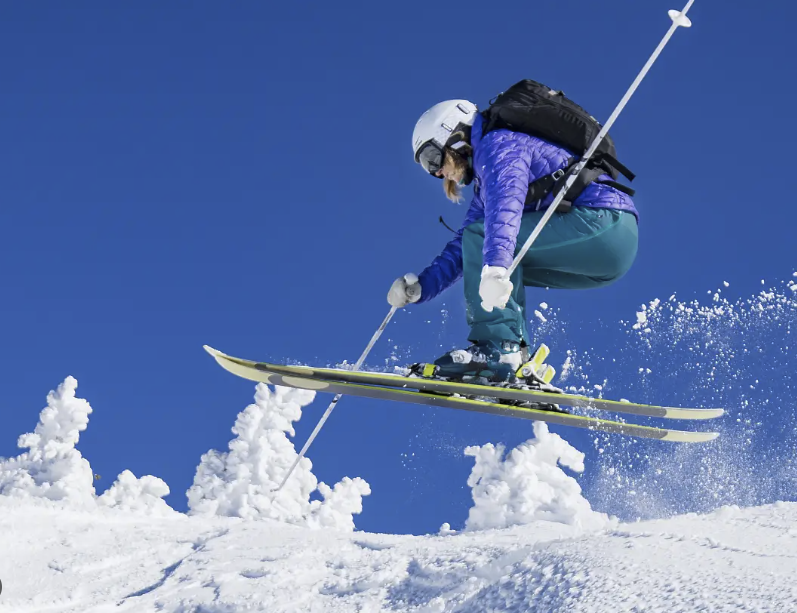
\includegraphics[width=0.9\textwidth]{assets/719dd84e.png}
            \par}
        \column{.5\textwidth}
        {\par\centering
            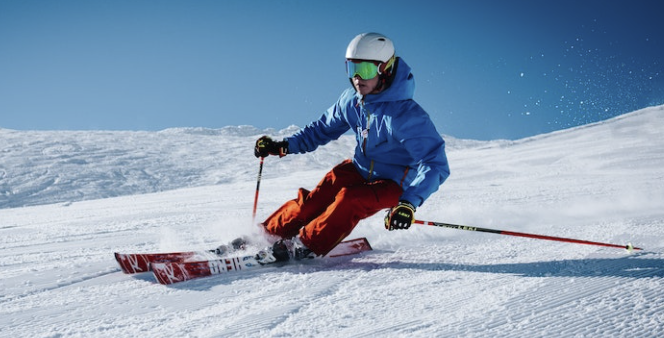
\includegraphics[width=0.9\textwidth]{assets/8e0a1697.png}
            \par}
    \end{columns}


\end{frame}

\begin{frame}{不倒翁roly poly toy}
    \par
    {\par\centering
        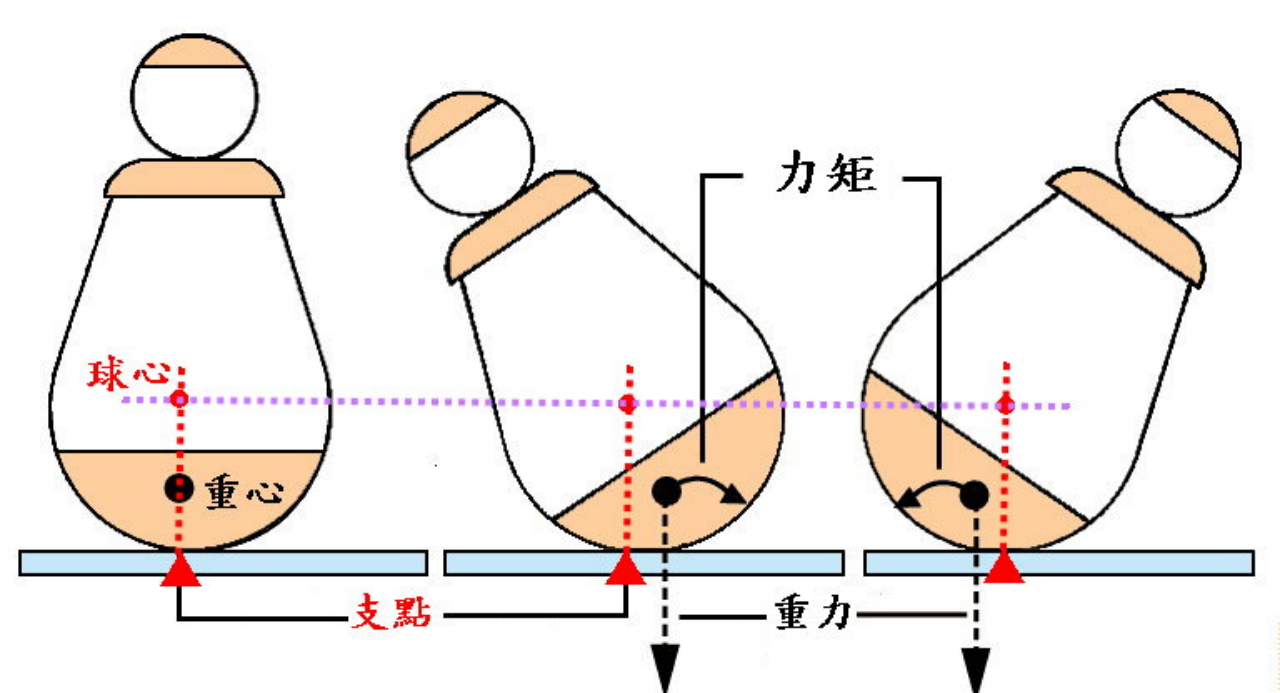
\includegraphics[width=.8\textwidth]{assets/c2d6f451.png}
        \par}
\end{frame}



\end{document}